\documentclass[a4paper]{article}
\usepackage{amsmath}

\usepackage{graphicx}
\graphicspath{{../analysis/}{../../analysis/}{../static/}{../../static/}}

\usepackage[round]{natbib}
\bibliographystyle{unsrtnat}

\usepackage{url}

\newcommand{\hii}{H\textsc{ii}~}
\newcommand{\cloudy}{{\tt CLOUDY}~}

\title{The Physics of \hii Regions}\label{the-physics-of-hii-regions}
\author{Josh Borrow}

\begin{document}

\maketitle

\section{Introduction}

In this problem, we model the \hii region of an O star, within a cloud of
Hydrogen and Helium. It is worth starting with a brief description of what a
\hii region is, where they are found, and how they play a role. In Figure
\ref{fig:hiidiagram} we show a schematic of the ISM extracted from
\citet{borrow_towards_2017}.

\begin{figure}[!h]
    \centering
    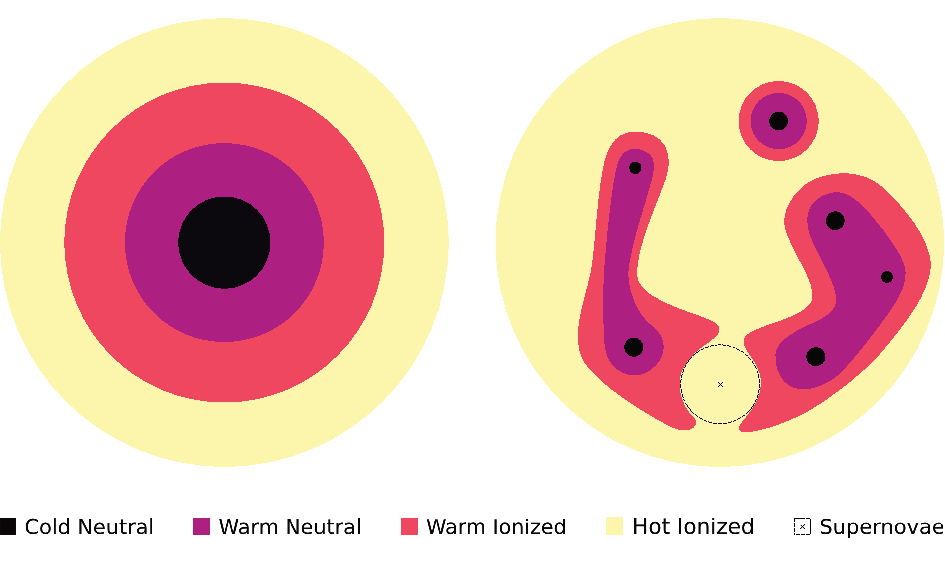
\includegraphics[width=\textwidth]{structure.pdf}
    \caption{The structure of the ISM. This is, in general, split up into four
        distinct parts in accordance with the work by
        \citet{mckee_theory_1977}.  The left image shows an isolated molecular
        cloud. The \hii region would correspond to the `ionised` regions around
        the central star forming `cold neutral' sphere. This is not the only
        time in which a \hii region forms, but in general they are found around
        collections of hot, young stars. On the right, a top-down image of the
        `large-scale' ISM is shown (around 1 kpc scale). It can be seen that
        multiple molecular clouds sit in the ISM, each surrounded by a large
        \hii region. Note that the \hii regions can be `joined'.}
    \label{fig:hiidiagram}
\end{figure}

\hii regions are associated with recent star formation
\citep{anderson_molecular_2009}, as is made clear by the schematic in Figure
\ref{fig:hiidiagram}.  They are formed primarily of ionised hydrogen, \hii, as
their name suggests, but are of course full of other ionised species as well,
such as He\textsc{ii}.  The temperature of these regions has been known to be
approximately $10^4$ K for many decades \citep{peimbert_temperature_1967}.

\section{Theoretical Study}

One of the first papers published on the theory behind \hii regions is
\citet{stromgren_physical_1939}. Due to their relative abundance in the solar
neighborhood, \hii regions have been well studied; as far back as 
\citep{struve_emission_1938} it has been theorised that they arise due to
hot O and B stars that are present in regions of recent star formation.

In \citet{stromgren_physical_1939} the author makes the following key
assertions:
\begin{itemize}
    \item At the centre of the \hii region, there should be a collection of
          stars that produce ionising radiation.
    \item The photons from the star will ionise the gas around them. This
          gas will eventually re-combine, but this will emit a photon that is
          capable of ionising \emph{another} hydrogen atom (perhaps
          behind the original atom), ensuring that the `ionisation front'
          will always progress away from the star.
    \item The sphere should be fully ionised due to the large amount of
          ionising radiation produced by the star(s) and the aforementioned
          `back-propagation' mechanism.
\end{itemize}
This leads naturally to the idea of a \citet{stromgren_physical_1939} sphere,
an ionised \hii region around a source of ionising photons. The sphere has
radius
\begin{align}
    R_S = \left(
    \frac{3}{4\pi} \frac{S_*}{n^2 \alpha} \right)^{1/3},
    \label{eqn:rs}
\end{align}
where $S_*$ is the luminosity of the central star in terms of photons per unit
time, $n$ is the number density of hydrogen in the cloud, and $\alpha
\approx 3\times 10^{-13}$ cm$^{4}$ s$^{-1}$ is the total recobination rate.

This is underlied by the following assumptions:
\begin{itemize}
    \item The density of hydrogen in the sphere is constant throughout, and
          the cloudy is composed solely of hydrogen.
    \item The number density of electrons in the sphere is the same as
          the number density of hydrogen nuclei.
    \item The sphere is fully ionised, and the boundary between the ionised
          region and the rest of the ISM is infinitely sharp.
    \item The \hii region is at a constant temperature of $10^{4}$ K.
\end{itemize}

In the section below, we will use the numerical radiative transfer code
\cloudy \citep{ferland_2017_2017} to assess if this theory produces
correct radii for \hii regions, and to interrogate the assumptions that the
above model makes.

\section{Numerical Study}

The \hii regions are now studied using the numerical radiative transfer code
\cloudy \citep{ferland_2017_2017}. In Table \ref{tab:sims} we list the
runs that were performed and hence what areas of parameter space were explored.

\begin{table}[!h]
    \centering
    \resizebox{\textwidth}{!}{
    \begin{tabular}{l|c|c|c|l}
        Run Name & Temperature (K) & Density ($n_H$ cm$^{-1}$) & $S_*$ & Notes \\
        \hline
        {\tt dens\_var} & $35\times10^4$ & $10^1$ - $10^5$ & $10^{49}$ & ISM abundances\\
        {\tt dens\_var\_only\_hydrogen} & $35\times10^4$ & $10^1$ - $10^5$ & $10^{49}$ & Abundances for all species: $10^{-18}$ \\
        {\tt qh\_var} & $35\times10^4$ & $10^2$ & $10^{47}$ - $10^{52}$ & ISM abundances\\
        {\tt temp\_var\_lowdensity} & $10$ - $100 \times 10^4$ & $10^1$ & $10^{49}$ & ISM abundances \\
        {\tt temp\_var\_highdensity} & $10$ - $100 \times 10^4$ & $10^3$ & $10^{49}$ & ISM abundances\\
    \end{tabular}}
    \caption{The runs presented below. Note that $S_*$ refers to the number of
        \emph{ionising} photons, i.e. this is {\tt q(h)} in the \cloudy code.}
    \label{tab:sims}
\end{table}
To compare our numerical runs with the theoretical predictions for the
\citet{stromgren_physical_1939} radius, we need to be able to extract the
cloud edge radius from from the simulation data. there are several ways to do
this, but here we choose to use the minimum of the derivative of the \hii
fraction (see Figure \ref{fig:derivative} for a pictorial version), as this
should be the turning point of the \hii curve. This will slightly
under-predict the cloud radius, but only if the transition between the cloud
and the rest of the ISM is not sharp. This turns out to be a reasonable
assumption for nearly all of the data collected (see figures below).

\begin{figure}[!h]
\centering
\includegraphics[width=\textwidth, trim=0.5cm 0.5cm 0.5cm 0.5cm]{differential.pdf}
\caption{First derivatives of the H$\textsc{ii}$ abundance with
respect to depth into cloud. The different lines correspond to different
black body temperatures for the central star, at a fixed density of
$n_H = 1\times 10^3$. It is clear from fig.~\ref{fig:density} that
there is a turning point in the H$\textsc{ii}$ abundance at what
appears to be the `edge' of the cloud. By using the minima of this
derivative we can find the edge programmatically.}\label{fig:derivative}
\end{figure}

\begin{figure}
\centering
\includegraphics[width=\textwidth, trim=1cm 1cm 1cm 1cm]{density.pdf}
\caption{The hydrogen, H$\textsc{i}$, and H$\textsc{ii}$ densities
are shown by the blue, orange, and green lines respectively. Note that
the different panels correspond to varying initial hydrogen density. It
is assumed that the cloud is equally dense throughout. The final panel
shows how the radius of the edge of the H$\textsc{ii}$ and
He$\textsc{ii}$ regions changes with cloud
density.}\label{fig:density}
\end{figure}


\section{Discussion}

\section{Codes}

You can find all of the codes, parameterfiles, and even the \LaTeX~ source
for this report in the following GitHub repository,
\url{https://github.com/JBorrow/cloudy-hii-regions-homework}.

\bibliography{library}

\end{document}
